%Generales 
\documentclass[letterpaper,12pt]{article} % Documento en dos columnas, tamaño carta
\usepackage[spanish]{babel}       % Traduce capítulos, fechas, etc. al español
\usepackage[utf8]{inputenc}       % Permite usar acentos directamente
\usepackage[T1]{fontenc}          % Codificación para que se vean bien los caracteres en PDF
\usepackage{lmodern}              % Usa fuentes escalables compatibles con microtype
\usepackage{geometry}             % Control de márgenes y tamaño de página
\usepackage{fancyhdr}            % Encabezados y pies de página personalizados

%Notación 

\usepackage{amsmath}  % Ecuaciones, símbolos y fuentes matemáticas
\usepackage{amssymb}
\usepackage{amsfonts}
\usepackage{siunitx}                     % Escritura coherente de unidades del SI y números

%gráficos 

\usepackage{graphicx}           % Insertar y escalar imágenes
\usepackage{subcaption}         % Subfiguras dentro de una figura
\usepackage{booktabs}           % Tablas más profesionales
\usepackage{longtable}          % Tablas que ocupan varias páginas
\usepackage{tabularx}           % Tablas con ancho ajustable automáticamente


% --- COLORES Y LISTAS PERSONALIZADAS ---
\usepackage{xcolor}             % Uso de colores en texto y figuras
\usepackage{enumitem}           % Listas personalizadas (espaciado, numeración)

% --- HIPERVÍNCULOS Y NAVEGACIÓN ---
\usepackage{hyperref}           % Enlaces ciclables en PDF (índice, URLs, referencias)

% --- DIAGRAMAS TÉCNICOS ---
\usepackage{tikz}                         % Gráficos vectoriales (bloques, flujos, redes)
\usepackage{forest}                      % Árboles, jerarquías (estructuras)

% --- ALGORITMOS Y CÓDIGO FUENTE ---
\usepackage{algorithm2e}    % Pseudocódigo paso a paso (algoritmos)
\usepackage{listings}       % Mostrar código fuente con formato

\geometry{letterpaper, margin=1in} % Márgenes de 1 pul
\title{Ayahuik 1: Guía de Misión}
\author{CUAUHTÉMOC IPN}


\pagestyle{fancy} 
\setlength{\headheight}{14.5pt}
\fancyhf{}
\fancyhead[C]{Cuauhtemoc IPN}
\fancyhead[R]{AYAHUIK 1}
\fancyhead[L]{Guia de Misión}
\fancyfoot[R]{\thepage}

\graphicspath{{Imagenes/}}

\begin{document}

\section{Antecedentes}

    \subsection{Antecedentes Históricos}

    \subsection{Antecedentes IPN}

    \subsection{Antecedentes Cuauhtémoc IPN}

\section{Descripción general de la misión}

    \subsection{Participantes de la misión}

    \subsection{CONOPS}

    \subsection{Descripción de la carga util}

    \subsection{Descripción del proceso de diseño y construcción}

    \subsection{Descripción del lanzamiento y recuperación}

\section{Objetivos y criterios de éxito}

    \subsection{Objetivos generales}

    \subsection{Objetivos específicos}
    
    \subsection{Criterios de éxito}

\section{Resultados esperados}

    \subsection{Resultados técnicos}

    \subsection{Resultados de la misión}

    \subsection{Resultados de la carga útil}
\newpage
\section{organización y roles}

    El equipo Cuauhtémoc IPN está organizado en diferentes subsecciones para asegurar el funcionamiento del equipo y una gestión 
    eficiente de las misión, todas estas seran coordinadas por los lideres de mision 
    y estos a su ves por los capitanes del equipo. 
    
    \subsection{Organización del equipo}

    \begin{figure}[!h]
      \centerline{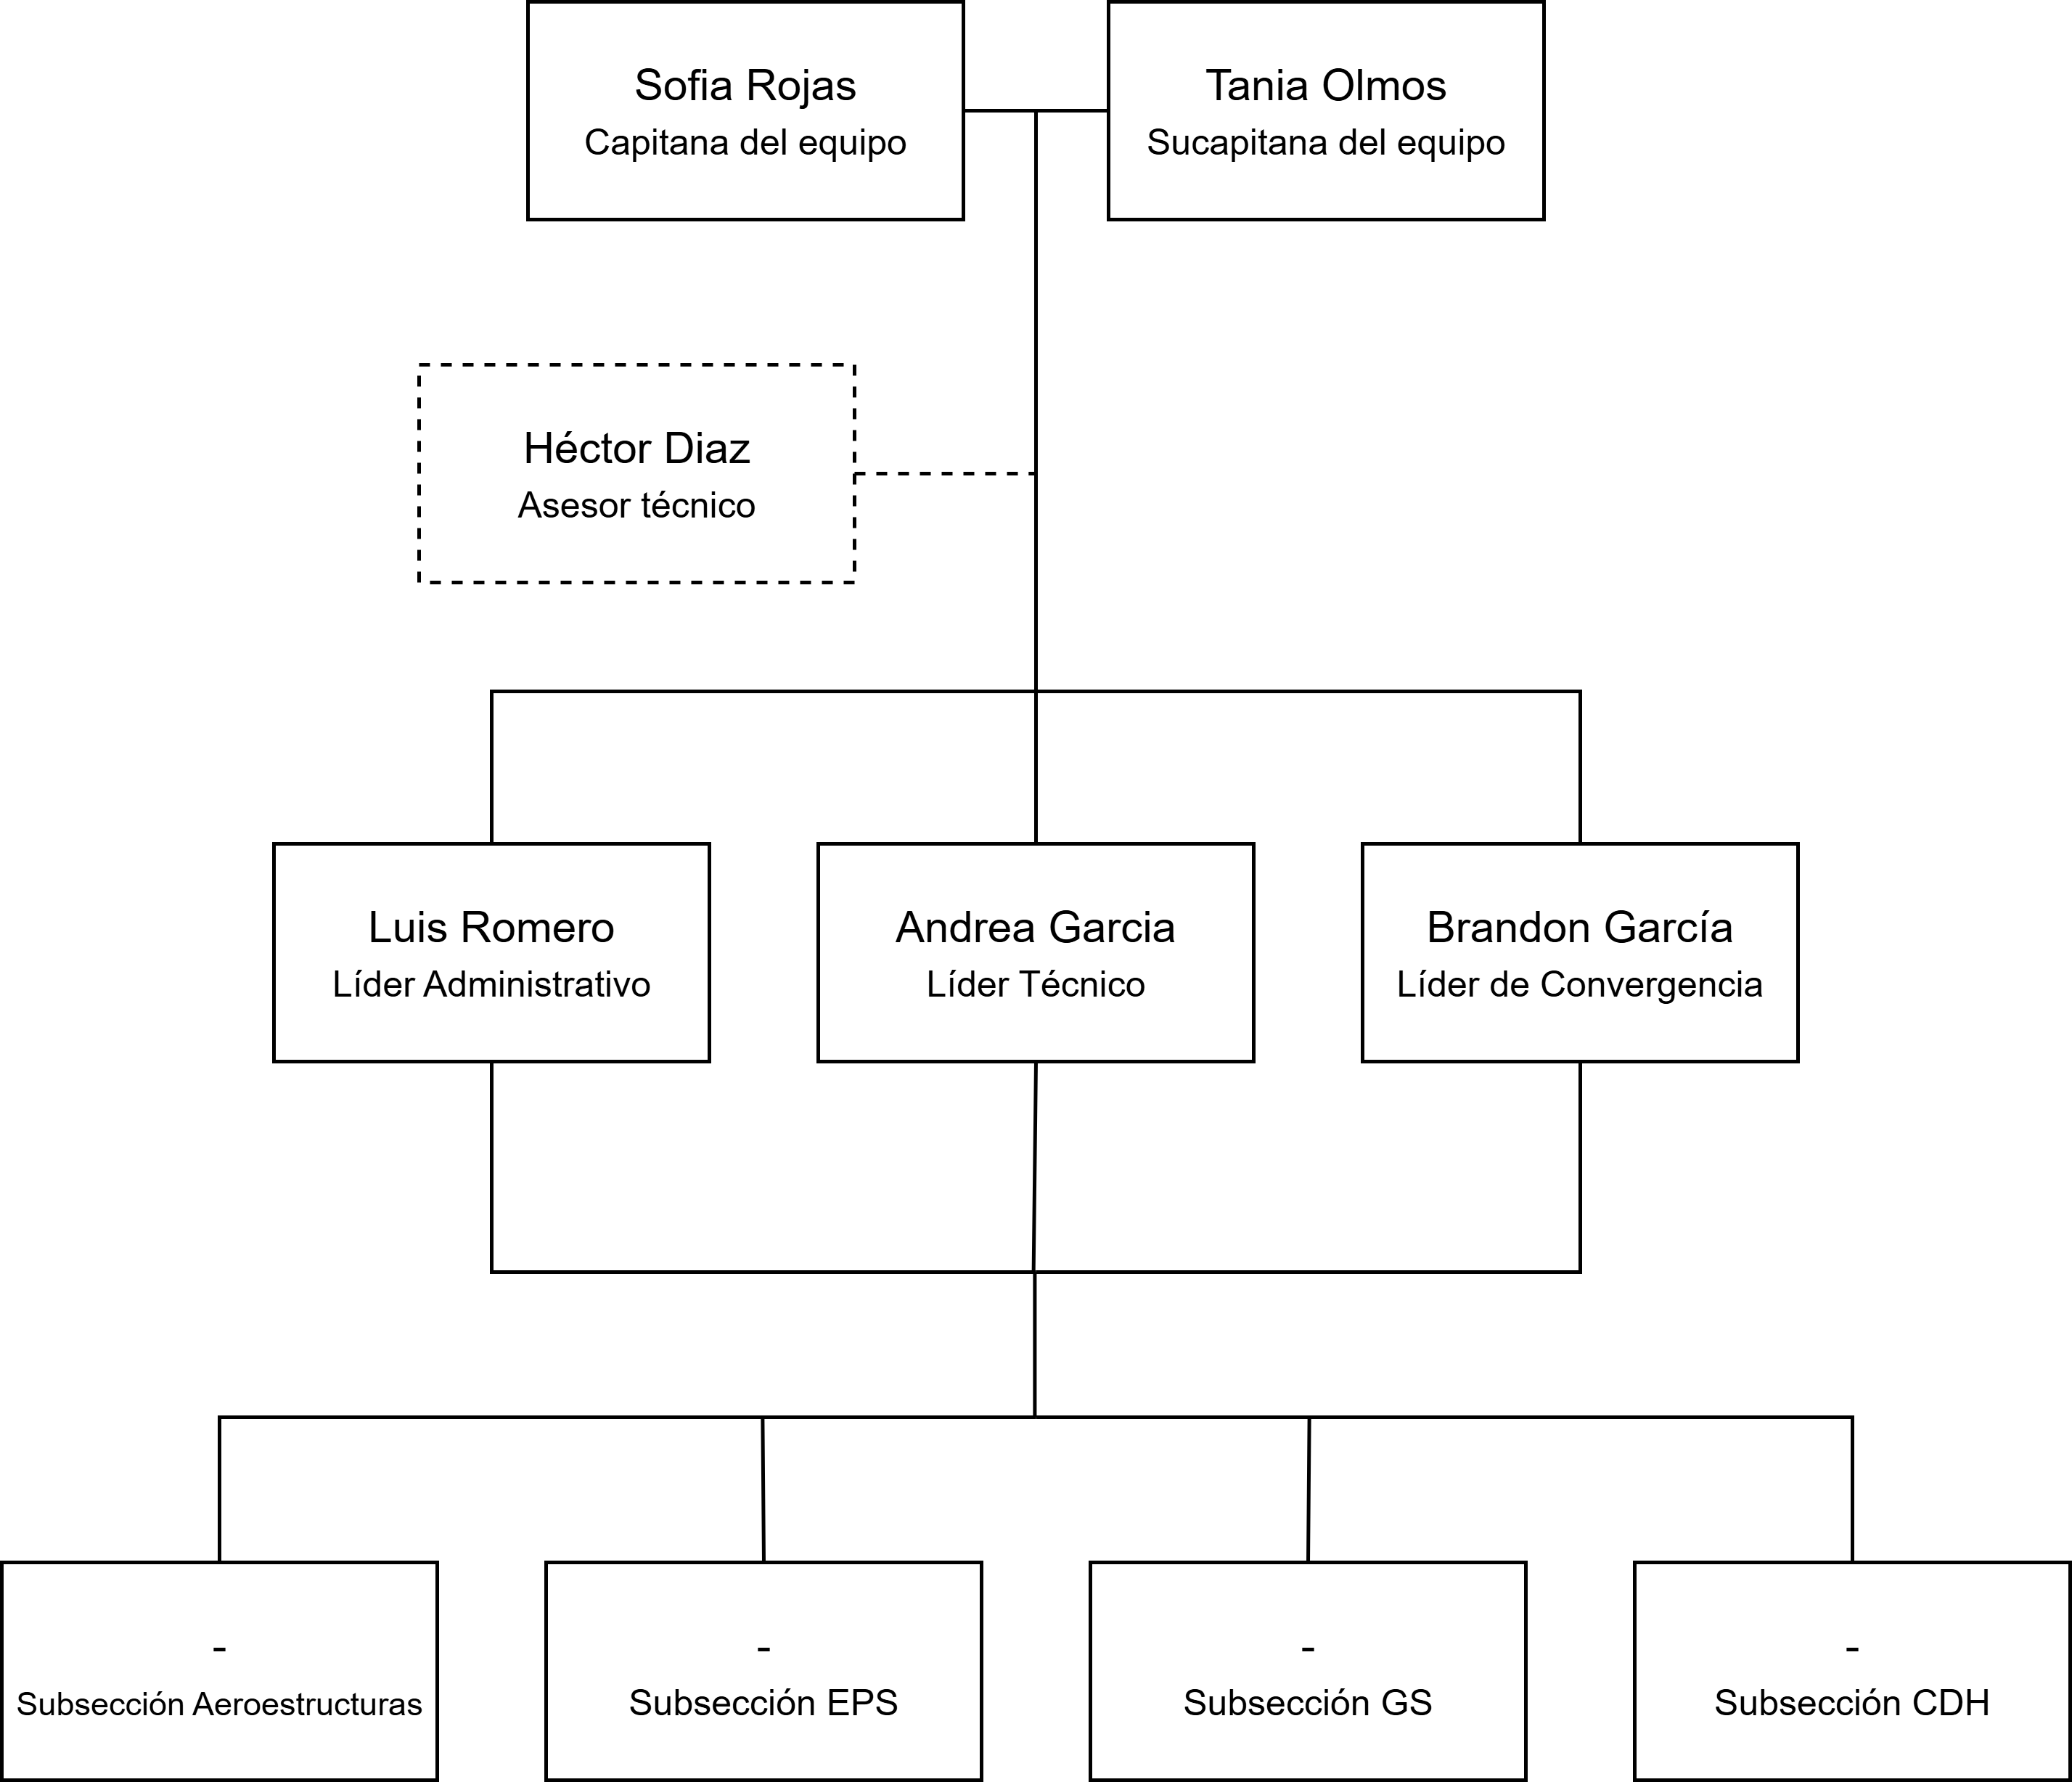
\includegraphics[width=.5\textwidth]{ORG-AYA1-GM.png}}
      \caption{Organigrama Ayahuik 1}
      \label{1}
    \end{figure}

    \subsection{Roles y responsabilidades}

\end{document}
